\documentclass[11pt,a4paper]{article}
\usepackage[utf8]{inputenc}
\usepackage[margin=2.3cm]{geometry}
\usepackage{amsmath}
\usepackage{graphicx}
\usepackage{booktabs}
\usepackage{xcolor}
\usepackage[font=small,labelfont=bf,skip=4pt]{caption}
\usepackage{float}
\usepackage{enumitem}
\usepackage{titlesec}

\definecolor{azul}{HTML}{1F4E79}
\titleformat{\section}{\large\bfseries\color{azul}}{\thesection}{0.6em}{}
\titlespacing*{\section}{0pt}{11pt}{5pt}
\setlist[itemize]{leftmargin=1.4em,topsep=3pt,itemsep=3pt,parsep=0pt}
\hyphenpenalty=10000 \exhyphenpenalty=10000 \sloppy
\setlength{\parskip}{4pt}
\renewcommand{\arraystretch}{1.15}
\renewcommand{\figurename}{Figura}
\renewcommand{\tablename}{Tabela}
\pagestyle{plain}

\begin{document}

\begin{center}
{\Large\bfseries\color{azul} Dá para prever o consumo de um carro?}\\[6pt]
{\small
UNINASSAU Teresina --- Análise e Desenvolvimento de Sistemas, 4º Período, Turma A\\
Machine Learning --- Prof. Dr. Alan da Silva Assunção\\[4pt]
\textit{Aluno:} João Paulo Oliveira da Silva\\[4pt]
Agosto de 2026}
\end{center}
\vspace{2pt}\hrule\vspace{4pt}

\section{O problema}

Carro pesado e potente gasta mais combustível isso todo mundo sabe. Queremos transformar essa ideia em número e prever o consumo de um carro só olhando suas características. Para isso usamos a \textbf{regressão linear}, que procura a reta que passa mais perto dos dados observados.

\begin{itemize}
  \item \textbf{O que queremos prever:} o consumo de combustível do carro.
  \item \textbf{Variável resposta ($Y$):} \texttt{mpg} (milhas por galão). Quanto maior, mais econômico o carro. É o nosso ``km por litro''.
  \item \textbf{Variáveis usadas para prever:} \texttt{wt} (peso) e \texttt{hp} (potência do motor).
  \item \textbf{Por que elas ajudam:} empurrar um carro pesado dá mais trabalho, e esse trabalho sai da queima de combustível. E um motor só entrega mais força porque consome mais combustível a cada explosão.
\end{itemize}

\section{Os dados}

Foi usado a base \texttt{mtcars}, que já vem instalada no R. Ela traz informações de \textbf{32 carros} fabricados entre 1973 e 1974, em \textbf{11 colunas}. Não falta nenhum dado.

\begin{table}[H]
\centering
\caption{Estatísticas das colunas usadas (32 carros).}
\small
\begin{tabular}{llrrrrr}
\toprule
\textbf{Coluna} & \textbf{Significado} & \textbf{Menor} & \textbf{Média} & \textbf{Maior} \\
\midrule
\texttt{mpg} & Consumo (milhas/galão) & 10,4 & 20,1 & 33,9 \\
\texttt{wt}  & Peso (mil libras)      & 1,51 & 3,22 & 5,42 \\
\texttt{hp}  & Potência (cavalos)     & 52 & 146,7 & 335 \\
\bottomrule
\end{tabular}
\end{table}

O carro mais econômico faz 33,9 mpg e o mais gastão faz 10,4 --- uma diferença de mais de três vezes. Medimos também a \textbf{correlação} de cada característica com o consumo, que mostra se elas andam juntas: peso deu $-0{,}87$ e potência $-0{,}78$. O sinal negativo confirma que, quando uma sobe, o consumo piora.

\section{Gráfico inicial}

A Figura 1 cruza o peso de cada carro com o seu consumo.

\begin{figure}[htbp]
\centering
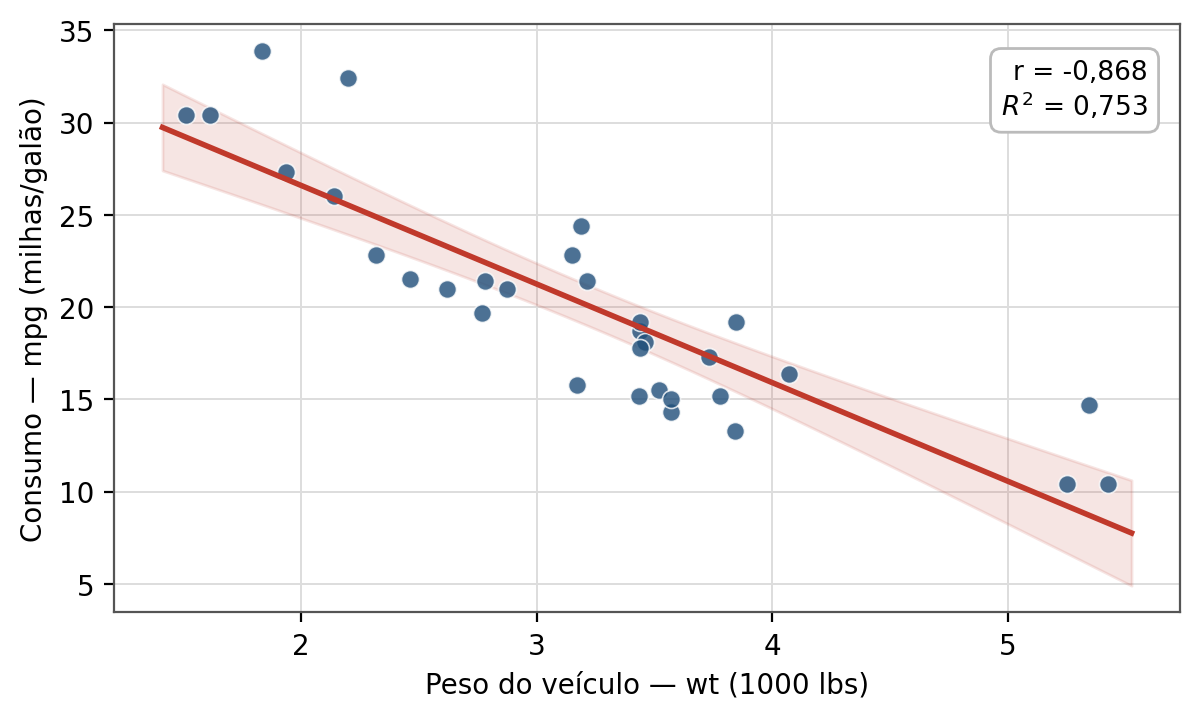
\includegraphics[width=0.68\textwidth]{fig1_dispersao.png}
\caption{Cada bolinha é um carro. Quanto mais à direita, mais pesado; quanto mais acima, mais econômico. A linha vermelha é a reta encontrada pelo modelo.}
\end{figure}

Na Figura 1, as bolinhas descem da esquerda para a direita e seguem um caminho parecido com uma linha reta. Isso confirma que quanto mais pesado o carro, menos ele anda por galão --- e que a regressão linear é adequada aqui.

\section{Regressão linear simples (só o peso)}

Comando no R: \texttt{lm(mpg \textasciitilde{} wt, data = mtcars)}. Resultado:

\[
\text{consumo previsto} = 37{,}2851 - 5{,}3445 \times \text{peso}
\]

\textbf{O 37,2851 ($\hat\beta_0$):} é o consumo previsto para um carro de peso zero. Como carro nenhum pesa zero, esse número não tem sentido prático --- ele só marca onde a reta começa no gráfico.

\textbf{O $-5{,}3445$ ($\hat\beta_1$):} a cada mil libras a mais de peso (cerca de 450 kg), o carro perde em média 5,34 milhas por galão. O sinal negativo confirma que mais peso significa mais consumo.

\textbf{$R^2$ ajustado $= 0{,}7446$.} Esse número vai de 0 a 1 e diz o quanto o modelo explica. Ou seja: \textbf{74\% das diferenças de consumo entre os carros são explicadas só pelo peso}.

\section{Regressão linear múltipla (peso + potência)}

Comando: \texttt{lm(mpg \textasciitilde{} wt + hp, data = mtcars)}. Resultado:

\[
\text{consumo previsto} = 37{,}2273 - 3{,}8778 \times \text{peso} - 0{,}0318 \times \text{potência}
\]

\textbf{Houve melhora? Sim.} O $R^2$ ajustado subiu de \textbf{0,7446} para \textbf{0,8148}: agora explicamos 81\% das diferenças de consumo, em vez de 74\%. Um teste feito no R confirmou que essa melhora é real, e não coincidência. A potência traz uma informação que o peso sozinho não dava.

\begin{table}[H]
\centering
\caption{Comparação dos dois modelos.}
\small
\begin{tabular}{lcc}
\toprule
\textbf{Modelo} & \textbf{$R^2$ ajustado} & \textbf{Quanto explica} \\
\midrule
Só peso & 0,7446 & 74\% \\
Peso + potência & \textbf{0,8148} & \textbf{81\%} \\
\bottomrule
\end{tabular}
\end{table}

\section{Treino e teste}

Avaliar o modelo nos mesmos carros que ele estudou seria como corrigir uma prova com o gabarito do próprio aluno. Por isso separamos os dados: \textbf{22 carros para treino} (70\%) e \textbf{10 para teste} (30\%), que o modelo nunca viu.

Treinando só com os 22 carros, o modelo ficou:
\[
\text{consumo previsto} = 38{,}4553 - 4{,}1089 \times \text{peso} - 0{,}0334 \times \text{potência}
\]

Depois pedimos que ele chutasse o consumo dos 10 carros guardados e comparamos com o valor real:

\begin{table}[H]
\centering
\caption{Erro do modelo nos 10 carros de teste.}
\small
\begin{tabular}{lc}
\toprule
\textbf{RMSE} & 2,060 mpg \\
\textbf{MAE} & 1,723 mpg \\
\bottomrule
\end{tabular}
\end{table}

O \textbf{MAE} é o erro médio: o modelo errou o consumo de cada carro por 1,72 mpg, para mais ou para menos. O \textbf{RMSE} é parecido, mas pune mais os erros grandes. Como o consumo médio desses carros é 17,96 mpg, errar 2,06 significa \textbf{errar cerca de 11\%} --- um resultado bom.

\section{Conclusão}

Sim, dá para prever o consumo de um carro. O peso sozinho já explica 74\% das diferenças; somando a potência, chegamos a 81\%, com erro médio de menos de 2 mpg em carros que o modelo nunca tinha visto. Vale lembrar que a base tem só 32 carros, todos dos anos 1970, então essas contas não valem para carros de hoje.

\vspace{4pt}\hrule\vspace{3pt}
{\footnotesize\textit{Análises feitas no R. Código completo no arquivo \texttt{trabalho\_ml\_regressao.R}.}}

\end{document}
